\documentclass{amia}
\usepackage{graphicx}
\usepackage[labelfont=bf]{caption}
\usepackage[superscript,nomove]{cite}
\usepackage{color}
\usepackage{soul}
\usepackage{multirow}
\renewcommand*{\thefootnote}{\alph{footnote}}

\begin{document}

\title{Deep Neural Architectures for Discourse Segmentation in E-Mail Based Behavioral Interventions}

\author{Mehedi Hasan, BS$^{1}$\footnote{Authors provided an equal contribution. \label{footnote1}}, Alexander Kotov, PhD$^{1}$\textsuperscript{\ref{footnote1}}, Sylvie Naar, PhD$^{2}$, Gwen L. Alexander, PhD$^{3}$, April Idalski Carcone, PhD$^{4}$}

\institutes{
$^1$Department of Computer Science, Wayne State University, Detroit, Michigan \\  
$^2$Center for Translational Behavioral Research, Department of Behavioral Sciences and Social Medicine, Florida State University, Tallahassee, Florida\\
$^3$Department of Public Health Sciences, Henry Ford Health System, Detroit, Michigan\\
$^4$Department of Family Medicine and Public Health Sciences, School of Medicine, Wayne State University, Detroit, Michigan\\
}

\maketitle

\noindent{\bf Abstract}
\textit{Communication science approaches to developing effective behavior interventions, such as motivational interviewing (MI), are limited by the traditionally manual qualitative coding of communication exchanges, which is a very resource-intensive and time-consuming process. This study focuses on the analysis of e-Coaching sessions, behavior interventions that are delivered via email and grounded in the principles of MI. A critical step towards automated annotation of e-Coaching communication exchanges is segmentation of emails into fragments that correspond to MI behaviors. This study formulates this task as a classification problem and proposes word embeddings, punctuation and part-of-speech features to address it. We experimented both with traditional machine learning method, conditional random fields (CRF) and deep learning methods, such as multilayer perceptrons (MLP), bidirectional recurrent neural networks (BRNN) and convolutional recurrent neural networks (CRNN). Results indicate that CRNN outperformed CRF, MLP and BRNN achieving 0.989 macro F1-score overall and 0.825 macro F1-score for detecting new segment.}

\section*{Introduction}
The emergence of e-Health technologies opened up new ways to deliver a variety of behavioral interventions to any demographic group of patients in any geographical location. Motivational interviewing (MI), an evidence-based communication technique to increase intrinsic motivation and self-efficacy for behavior change,\cite{miller2012motivational,miller2009toward} is one type of these interventions. MI sessions are generally aimed at eliciting ``change talk'', or statements of intrinsic motivation about patients' own desire, ability, reasons, need for and commitment to behavior change, which have been established by previous research\cite{apodaca2009mechanisms} as a reliable mediator of health behavior change. \hl{However, communication science approaches to understanding the efficacy of MI are inherently limited by traditional qualitative coding methods}. 

Qualitative analysis of motivational interviews has been traditionally performed manually by MI researchers, which is a tedious and resource-intensive process involving several iterations of reading, comprehension and interpretation of interview transcripts. Rapidly developing computational technologies, specifically, machine learning methods, offer a unique opportunity to accelerate this process. In particular, machine learning methods have been successfully applied to a variety of analytical tasks involving textual data, such as classification\cite{nigam2000text} and sentiment analysis.\cite{wang2012baselines} In our previous work, we examined the utility of machine learning methods for automated annotation \cite{hasan2016study,kotov2015interpretable} and predicting the outcome \cite{hasan2018predicting} of in-person MI sessions. Experimental data utilized in these studies, however, were transcribed auto recordings of in-person MI sessions with a counselor, which have a clear discourse structure and were clearly segmented into the utterances by a counselor, a patient or a caregiver. 

In this study, we focus on the analysis of e-Coaching sessions, behavioral interventions that are delivered via email and are grounded in the principles of MI. Specifically, the e-Coaches involved in this study used emails to communicate motivation-enhancing messages that encourage healthy eating among GenY adolescents. E-coaching data is comprised of email responses, which are free-text documents, unlike more traditional dyadic clinical interviews that are naturally segmented into utterances due to their conversational nature.

The unstructured nature of e-Coaching exchanges poses a unique set of challenges for their qualitative analysis. Usually, email segments are automatically coded with the Minority Youth-Sequential Coding of Process Exchanges (MYSCOPE), \cite{carcone2013provider} a qualitative coding scheme to characterize patient-provider communication during MI session. A significant barrier to qualitative analysis of e-Coaching exchanges is their segmentation into textual fragments that correspond to a distinct e-Coach and patient communication behaviors. Automating this task is a unique and challenging problem due to the following reasons:

\begin{enumerate}
\item Emails are unstructured text containing informal information exchange in a non-traditional format. For example, an e-Coach usually responds to several previous patient statements in one email. However, in a traditional MI interview session involving a dialogue between a provider and a patient, a provider utterance is a response to an immediately preceding inquiry or statement by a patient. 
\item Discourse segments in e-Coaching emails do not necessarily correspond to sentences or paragraphs. One sentence can be divided into fragments corresponding to multiple MI behaviors. On the other hand, an MI behavior may comprise several sentences.
\end{enumerate}

\begin{figure}[!htb]
    \centering
    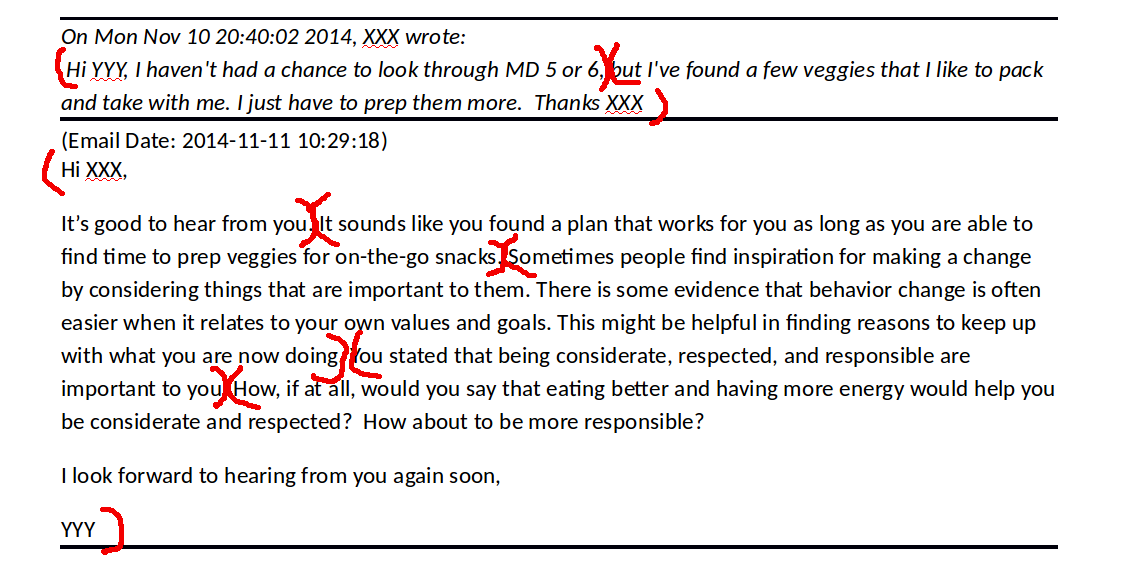
\includegraphics[width=0.7\textwidth]{figures/segment-example.png}
    \caption{\textbf{Example of e-Coaching emails segmented into fragments that correspond to MI behaviors of an e-Coach and a patient}}
    \label{fig:text-segment}
\end{figure}

Figure~\ref{fig:text-segment} illustrates a segmentation of an e-Coaching email exchange, in which the first sentence is segmented into 2 MI behavior fragments, while the fourth and fifth segments correspond to one and three sentences, respectively. Segmentation of e-Coaching email exchanges between patients and e-Coaches corresponds to a special case of discourse analysis \cite{webber2012discourse} aimed at better understanding the effective communication strategies specific to this type of behavioral interventions and revealing the unique socio-psychological characteristics of patients. 

The goal of this study is to assess the effectiveness of deep learning methods for the task of automated segmentation of e-Coaching emails into textual fragments corresponding to individual behaviors, which is the first step of qualitative analysis of this type of clinical communications. \hl {Specifically, for this study, we utilized the data from MENU GenY (Making Effective Nutrition Choices for Generation Y) }\cite{alexander2017motivations}, a recent technology-based public health intervention that relies on personalized e-Coaching to encourage increased fruit and vegetable intake among young adults, aged 21--30. The goal of MENU GenY was to develop a better coding scheme for e-Coaching communications aimed at improving GenY eating habits. Segmentation of clinical conversation in the context of electronically delivered interventions into groups of MI behaviors, is traditionally performed manually by MI researchers, which significantly slows down their qualitative analysis. This paper is the first work to evaluate the empirical effectiveness of deep learning architectures in addressing \textit{the problem of discourse segmentation in the context of e-mail based behavioral interventions}. 

Specifically, we introduce and evaluate the effectiveness of word embedding or lexical, punctuation and part-of-speech (POS) features in conjunction with both traditional supervised machine learning methods, such as linear-chain Conditional Random Field (CRF)\cite{lafferty2001conditional} and deep learning architectures, such as Multi-Layer Perceptron (MLP),\cite{rumelhart1986learning} Bidirectional Recurrent Neural Network (BRNN)\cite{schuster1997bidirectional} and Convolutional Recurrent Neural Network (CRNN),\cite{treviso2017sentence} to find the best performing method and feature combination. 

\section*{Relevant work}
Previous relevant work in the biomedical domain primarily focused on segmentation of text in electronic health records (EHR) into sections and headers \cite{apostolova2009automatic,denny2009evaluation,tepper2012statistical,cho2002text} or sentence boundary detection.\cite{griffis2016quantitative,kreuzthaler2015detection,treviso2017sentence} In particular, Maximum Entropy models \cite{tepper2012statistical} and Support Vector Machine (SVM) along with word-vector cosine similarity metric and several heuristics \cite{apostolova2009automatic} have been applied to segment or classify clinical documents in EHR into pre-defined sections, such as general patient information, medical history, procedures, findings, etc. Denny et al. \cite{denny2009evaluation} proposed a SecTag algorithm, which combined natural language processing techniques, terminology-based rules and a Naive Bayes classifier to identify sections and headers in EHR. Segmentation of e-Coaching emails, however, is different from segmentation of other clinical documents in that the focus is on clinical conversation.   

SVM in conjunction with prosodic and part of speech features \cite{kreuzthaler2015detection} and Recurrent Convolutional Neural Networks \cite{griffis2016quantitative} have also been utilized for \textit{sentence boundary detection} in general text. Liu et al. \cite{liu2005using} demonstrated that a linear-chain CRF outperforms Hidden Markov and Maximum Entropy models for this task. 

Segmentation of e-Coaching emails is different from a traditional shallow discourse analysis of conversations \cite{galley2003discourse} in that the focus is on segmentation, rather than on determining the types of transitions between the utterances or assigning utterances to speakers. The proposed methods will automate the process of segmenting clinical exchanges into groups of MI behaviors, which will significantly reduce the resources and time required to perform this task manually. Furthermore, these methods can be integrated with auto coding methods \cite{hasan2016study,kotov2015interpretable} to create a software pipeline for automated analysis of clinical conversation.
  
\section*{Methods}
\subsection*{\textit{Data collection}}
\hl{The experimental dataset for this work was constructed from 49 e-Coaching sessions, which include a total of 3,138 segmented and annotated MI behaviors. Each session represents an MI intervention delivered via email. We consider segmentation as a binary classification problem, in which each word or punctuation mark is annotated with a label of 1 or 0 to indicate whether it precedes a new segment or not. In total, the dataset consists of 95,777 words and 7,140 punctuation marks and includes 3,138 ``new segment'' and 99,779 ``same segment'' instances}. In this study, we experimented with traditional machine learning methods, such as Conditional Random Field (CRF)\cite{lafferty2001conditional} and deep learning methods, such as Multi-Layer Perceptron (MLP),\cite{rumelhart1986learning} Bidirectional Recurrent Neural Network (bidirectional RNN or BRNN)\cite{schuster1997bidirectional} and Convolutional Recurrent Neural Network (CRNN).\cite{treviso2017sentence} For an MLP model, training and testing instances were created based on a sliding window of $2n$ words or punctuation marks over each position in a given input sequence, such that each instance consists of a pair of the next $n$ words or punctuation marks and prior $n$ words or punctuation marks, including the current word or punctuation mark. Each sample is classified into either a ``new segment'' or a ``same segment'' based on whether there should be a segment break after the current word or not. In the case of CRF, BRNN and CRNN models, an email was taken as an input sequence, POS tags and word embeddings of each word or punctuation mark were used as input and binary labels (1 or 0) corresponding to ``new segment'' and ``same segment'' classification decisions were considered as the model output of a model. In the gold standard, words or punctuations within the same segment were assigned the label of 0 and the last word or punctuation mark of a segment were assigned the label of 1.     

\subsection*{\textit{Features}}

We utilized three types of features in conjunction with CRF, MLP, BRNN and CRNN methods: word embeddings or lexical features, punctuation and POS features. Since POS tags have been shown to be effective semantic abstractions of individual words, we used POS features for our experiment.\cite{liu2005using,treviso2017sentence} To extract POS features, we pre-processed e-Coaching emails using the NLTK POS tagger. Punctuation marks, which correspond to one of the symbols \{`.', `,', `!', `?', `:', `;'\} between a pair of words, were also used as a feature, since punctuation marks designate the boundary of a sentence, clause and phrase and often also correspond to a segment boundary.\cite{cho2002text} For natural language processing (NLP) tasks, inputs are received as a text, in which individual words are as the basic units of semantics. Therefore, it is important to represent a word in such a way that it carries all relevant information. Word embedding is one such representation, when each word is associated with a real-valued vector in a high dimensional vector space. Distributed representations of words have been shown to capture semantic, syntactic and morphological properties of words.\cite{pennington2014glove, mikolov2013distributed} For experiments reported in this paper, we utilized embeddings estimated on Google News corpus consisting of 1.6 billion words pre-trained using word2vec word embedding method.\footnote{\label{fn:word2vec}https://code.google.com/p/word2vec/} When words or punctuation marks are not found in the pre-trained word vectors, we utilized word embeddings trained with our e-Coaching email corpus, which we refer to as corpus-based embeddings. CRF utilized lexical features, which correspond to words in e-Coaching emails. 

\subsection*{\textit{Classifiers}}

We experimented with 4 different classifiers, including one traditional machine learning method, CRF and three deep learning models. Since deep learning architectures provide a flexible mechanism for constructing complex models, we take the advantage of this flexibility to test MLP, BRNN and CRNN models for the task of segmentation of e-Coaching emails.

\textbf{Conditional Random Field}: CRF has been widely used in various NLP tasks, such as part-of-speech tagging.\cite{lafferty2001conditional, hirohata2008identifying} Unlike a maximum entropy Markov model, which uses per-state exponential models for conditional probability of the next state given a current state, CRF model directly estimates conditional distribution of the entire output sequence, given the observation sequence. A traditional linear-chain CRF model is defined as a conditional probability distribution $p(y|x)$ for output and input sequences, $y$ and $x$:

\begin{equation}
\label{Eq:crf}
p(y|x) = \frac{1}{Z_x}\exp{\left(\sum_{t=1}^{T}\sum_{k}^{}\lambda_k f_k(y_{t-1}, y_t, x, t)\right)} \\
\end{equation}

where $Z_x$ is a normalization factor, $f_k(y_{t-1}, y_t, x, t)$ is a feature function, and $\lambda_k$ is a learned weight associated with feature $f_k$. The optimal output sequence $y^*$ for an input sequence $x$, $y^* = {arg\,max}_y p(y|x)$, is obtained efficiently using the Viterbi algorithm. In our experiments, the following features were utilized in conjunction with CRF models: i) current word or punctuation ii) next and previous 3 words or punctuations iii) binary feature indicating whether a word or punctuation is a special character (';', '?', '.', ',', '!', ':', etc.) or not iv) binary feature indicating whether a word is a title word or not (e.g. ``The'' is a title word but ``the'' is not) v) POS tags   

\begin{figure}[!htb]
    \centering
    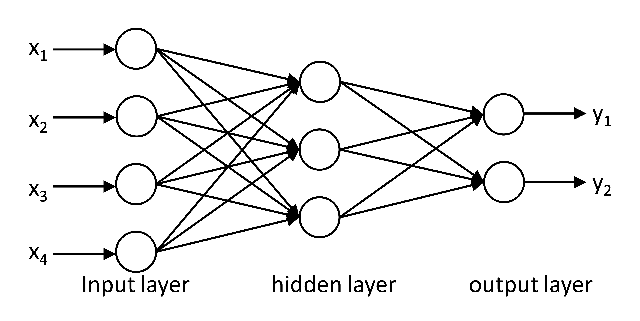
\includegraphics[width=0.45\textwidth]{figures/mlp.eps}
    \caption{\textbf{A multilayer perceptron with a single hidden layer}}
    \label{fig:mlp}
\end{figure}

\textbf{Multi-Layer Perceptron}: MLP is a feed-forward artificial neural network, which maps an input onto one or several outputs.\cite{rumelhart1986learning} Figure~\ref{fig:mlp} shows a multilayer perceptron with a single hidden layer. In MLP networks, there is no cycle or loop and information moves forward only, from the input nodes through the hidden nodes and to the output nodes. This study utilized MLP with a nonlinear activation function (rectified linear unit) and one hidden layer consisting of 128 hidden units. In order to prevent over-fitting, we utilized dropout in fully connected layers by randomly hiding neurons during training. \cite{srivastava2014dropout} Dropout is also applied to the fully connected layers in BRNN and CRNN models. 

\textbf{Bidirectional Recurrent Neural Network}: BRNN is a neural network designed to capture sequential patterns by considering both past \& future inputs as well as complex relationships between input features and output labels.\cite{schuster1997bidirectional} The output of BRNN layer is computed as an aggregation of outputs of the forward and backward RNNs. Gated Recurrent Units (GRU)\cite{chung2014empirical} capable of handling variable size input sequence and having internal memory, which can be reset, were utilized as an RNN. Figure~\ref{fig:crnn} represents the architecture of BRNN, in the case when a convolution layer is removed.   

\textbf{Convolutional Recurrent Neural Network}: CRNN is a deep neural network architecture,\cite{treviso2017sentence} shown in Figure~\ref{fig:crnn}, \hl {which consists of 5 layers: 1) input layer 2) embedding layer 3) convolution layer with max pooling 4) BRNN layer 5) fully connected layer with dropout and sigmoid output. 
E-coaching email exchanges are represented as a sequence of $m$ words and punctuations, which are fed into the input layer to produce a $m \times n_e$ matrix after fetching the pre-trained word vectors. When POS tags are used in combination with word embeddings, 10-dimensional POS vectors are concatenated with 300-dimensional word vectors to obtain new vectors $n_e = [n_w;n_p]$ of size 310. The primary purpose of convolution is to extract new features depending on the neighboring words. We used 1D convolution. In this layer, one filter is responsible for extraction of one feature. After applying $n_f$ different filters with zero-padding on both sides of the input text, $n_f$ useful features are produced in the convolution layer for each word. A max pooling operation was then performed over time to find the most significant features in a textual fragment. The bidirectional recurrent layer receives new features extracted in the convolution layer. RNN is usually used to capture long-range dependencies in a sequence of observations. Moreover, bidirectional RNNs are capable of capturing both past and future contexts through forward and backward traversals of a sequence. The purpose of the fully connected layer is to use the output of bidirectional RNN layer for classifying each word or punctuation into ``new segment'' and ``same segment'' classes. Since a fully connected layer has a greater number of parameters, they are more likely to excessively co-adapt with these parameters, which may cause over-fitting. To prevent this, we utilized dropout by randomly disregarding 50\% of the connections to the fully connected layer. After that, logistic sigmoid is applied to the output layer to provide the probability of whether the word or punctuation precedes a new segment or not}. We experimentally determined the optimal parameters and found that the best performance is achieved with 5-fold cross-validation when filter length in convolutional layer is 7, number of filters is 100, max-pool size is 3, ReLU is used as a convolutional layer activation function, RNN layer activation is hyperbolic tangent and the number of recurrent units in RNN is 200. Adam\cite{kingma2014adam} with 50 epochs, the batch size of 32 and learning rate of 0.001 was used for optimization and the early stopping strategy was applied.\footnote{\hl {source code will be available at https://github.com/teanalab/xxxxx upon acceptance of this paper for publication}}

\begin{figure}[!htb]
    \centering
    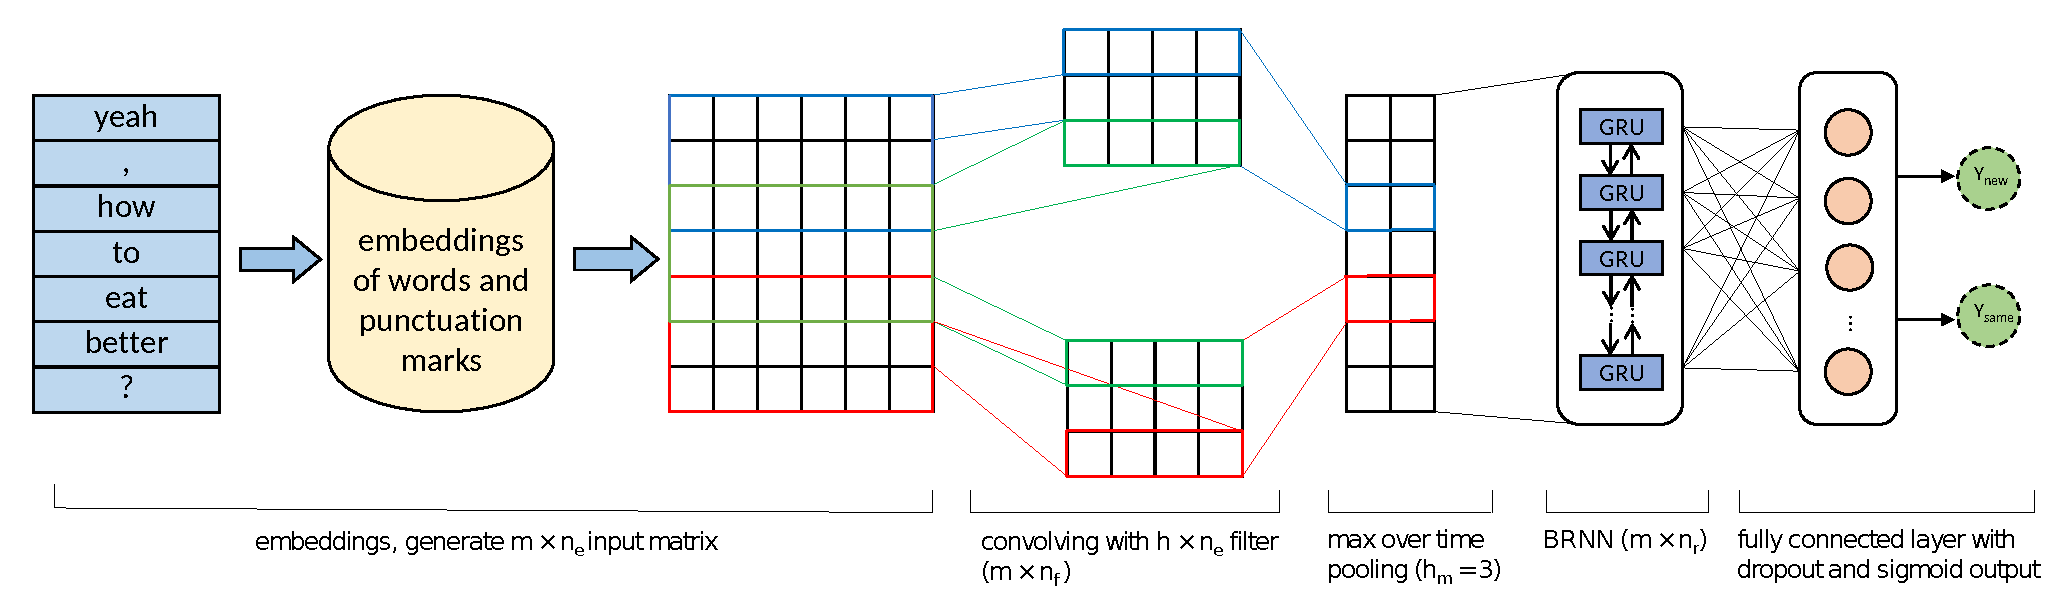
\includegraphics[width=0.95\textwidth]{figures/CRNN.eps}
    \caption{\textbf{Architecture of convolutional recurrent neural networks for automatic segmentation of e-Coaching emails}}
    \label{fig:crnn}
\end{figure}
  
\subsection*{\textit{Evaluation metrics}}
We report standard metrics of precision, recall and F1-measure to evaluate the performance of the classifiers.\cite{aas1999text} Accuracy is not reported as a performance metric because it is highly sensitive to the prior class probabilities and does not fully describe the actual difficulty of the decision problem, when highly unbalanced datasets are involved. The results are reported based on 5 fold cross-validation and weighted macro-averaging over the folds. \hl{We also estimate the area under the receiving operating characteristics (ROC) curve} \cite{kumar2011receiver} \hl{(AUC) metric due to its effectiveness in measuring the quality of binary classifiers for imbalanced datasets}. \cite{hu2015kernelized}

\section*{Results}
Our experiments span four dimensions. First, we report the optimal size of word embeddings and sliding window size of the MLP model. Second, results are reported with respect to ``new segment'' class as well as weighted average over ``new segment'' and ``same segment'' classes in Table~\ref{tab:result_base}. Third, classification performance of different machine learning methods are summarized in Table~\ref{tab:result_weighted_avg} when word embeddings or lexical features are used in combination with punctuation and POS features. Fourth, the impact of the individual features, as well as their combination on the segmentation task, is reported.

\begin{figure}[!htb]
    \centering
    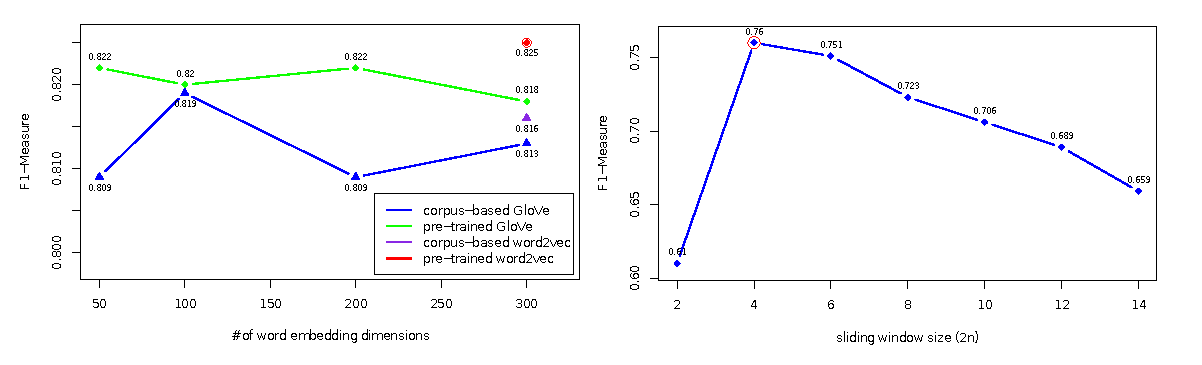
\includegraphics[width=0.95\textwidth]{figures/mlp-and-vector.eps}
    \caption{\textbf{Performance of CRNN model on e-Coaching email segmentation by varying the dimension of pre-trained and corpus word embeddings with GloVe and word2vec models (left). MLP model on e-Coaching email segmentation by varying the sliding window size 2n (right).}}
    \label{fig:embedding-dimension-mlp}
\end{figure}   

Figure~\ref{fig:embedding-dimension-mlp} (left) shows the performance of CRNN model on e-Coaching email segmentation by varying the dimension of pre-trained and corpus word embeddings with GloVe \footnote{https://nlp.stanford.edu/projects/glove/} and word2vec models. It was observed that best performance is achieved with pre-trained 300-dimensional word2vec word vectors when three types of features are used together. Therefore, we report our results with word2vec 300-dimensional word vectors for all deep learning models used in this study. For MLP models, the first layer input was prepared by the summation of the first $n$ word vectors in the sliding window and the last $n$ word vectors when a sliding window contains $2n$ words or punctuations. Figure~\ref{fig:embedding-dimension-mlp} (right) demonstrates the performance of the MLP model on e-Coaching email segmentation by varying the size of the sliding window. It can be observed that the best performance of MLP is achieved when $n$ is 2. Therefore, results of MLP in the remaining experiments are reported with $n$ set to 2. 

As follows from Table~\ref{tab:result_base}, CRNN outperforms all other models in terms of recall and F1-measure achieving 0.797 recall with 0.785 F1-measure for new segment detection. CRNN also shows superior performance in all performance metrics for weighted average over ``new segment'' and ``same segment'' classes. BRNN demonstrates the lowest performance among all models in terms of precision and F1-Measure. On the other hand, MLP has the highest precision of 0.836 when word embeddings or lexical features are used to identify ``new segment''. CRF achieves 0.733 F1-Measure in new segment class and 0.984 F1-Measure overall, which corresponds to the second highest performance in identifying ``new segment'' as well as a weighted average over both classes. Experimental results indicate that performance of all classifiers as a weighted average over both classes is remarkably higher compared to ``new segment'' class, which is expected since 96.95\% of instances belong to the ``same segment'' class and 99.3\% of them are correctly classified. For example, as a weighted average over ``new segment'' and ``same segment'' classes, CRNN achieves 27.23\%, 23.71\% and 25.61\% higher precision, recall and F1-measure, respectively, compared to the ``new segment'' detection. 

\begin{table}[ht]
\centering
\caption{\textbf{Performance of CRF, MLP, BRNN and CRNN methods for identification of ``new segment'' class as well as weighted average over ``new segment'' and ``same segment'' classes when word embeddings or lexical features are used. The highest value for each performance metric is highlighted in bold.}}
\label{tab:result_base}
  \begin{tabular}{|l|l|l|l|l|l|l|}
  \hline
   \multirow{2}{*}{\textbf{Method}} & \multicolumn{3}{|c|}{\textbf{New Segment}} & \multicolumn{3}{|c|}{\textbf{Overall}} \\\cline{2-7}
   & \textbf{Precision}  & \textbf{Recall} & \textbf{F1-Measure} & \textbf{Precision}  & \textbf{Recall} & \textbf{F1-Measure} \\ \hline    
 CRF & 0.782 & 0.691 & 0.733 & 0.983 & 0.984 & 0.984 \\ \hline
 MLP & \textbf{0.836} & 0.593 & 0.694 & 0.982 & 0.983 & 0.982 \\ \hline
 BRNN & 0.606 & 0.680 & 0.641 & 0.977 & 0.976 & 0.976 \\ \hline
 CRNN & 0.775 & \textbf{0.797} & \textbf{0.785} & \textbf{0.986} & \textbf{0.986} & \textbf{0.986} \\ \hline
  \end{tabular}
\end{table}                              

Table~\ref{tab:result_weighted_avg} summarizes the results of all models for segmentation of e-Coaching emails when word embeddings or lexical features are used in combination with punctuation and POS features. Similar to results in Tables~\ref{tab:result_base}, CRNN demonstrates the highest performance among all methods achieving 0.864 recall with 0.825 F1-Measure for ``new segment'' detection and 0.990 precision with 0.989 recall and F1-Measure overall. BRNN and CRF show the lowest and second highest performance, respectively, for email segmentation among all methods. We observed that classification performance significantly improved for ``new segment'' class when word embeddings or lexical features are used in combination with punctuation and POS features. Precision increases by 3.96\%, -2.27\%, 12.71\% and 1.81\%; recall increases by 11.72\%, 19.73\%, 20.59\% and 8.41\%; and F1-measure increases by 8.05\%, 9.51\%, 16.22\% and 5.1\% for CRF, MLP, BRNN and CRNN methods, respectively, in new segment detection when all features are utilized together. Similarly, precision increases by 0.51\%, 0.41\%, 0.82\% and 0.41\%; recall increases by 0.41\%, 0.41\%, 0.72\% and 0.3\%; and F1-measure increases by 0.41\%, 0.41\%, 0.82\% and 0.3\% for CRF, MLP, BRNN and CRNN methods, respectively, in weighted average over ``new segment'' and ``same segment'' classes when word embeddings or lexical features are used in combination with punctuation and POS features.\\

\begin{table}[ht]
\centering
\caption{\textbf{Performance of CRF, MLP, BRNN and CRNN methods for identification of ``new segment'' class as well as weighted average over ``new segment'' and ``same segment'' classes when all features are used together. The highest value for each performance metric
is highlighted in bold.}}
\label{tab:result_weighted_avg}
 \begin{tabular}{|l|l|l|l|l|l|l|}
  \hline
   \multirow{2}{*}{\textbf{Method}} & \multicolumn{3}{|c|}{\textbf{New Segment}} & \multicolumn{3}{|c|}{\textbf{Overall}} \\\cline{2-7}
   & \textbf{Precision}  & \textbf{Recall} & \textbf{F1-Measure} & \textbf{Precision}  & \textbf{Recall} & \textbf{F1-Measure} \\ \hline    
 CRF & 0.813 & 0.772 & 0.792 & 0.988 & 0.988 & 0.988 \\ \hline
 MLP & \textbf{0.817} & 0.710 & 0.760 & 0.986 & 0.987 & 0.986 \\ \hline
 BRNN & 0.683 & 0.820 & 0.745 & 0.985 & 0.983 & 0.984 \\ \hline
 CRNN & 0.789 & \textbf{0.864} & \textbf{0.825} & \textbf{0.990} & \textbf{0.989} & \textbf{0.989} \\ \hline
  \end{tabular}
\end{table}       

Table~\ref{tab:result_roc} \hl {shows the impact of individual features as well as their combination on the segmentation task. Although CRF provides the second highest classification results, it shows best AUC values, achieving AUC 0.966 when only lexical features are used and AUC 0.994 when a combination of lexical, punctuation and POS features are used. Influence of the punctuation and POS features is also consistent in AUC values, which increase by 2.9\%, 4.31\%, 6.63\% and 2.18\% for CRF, MLP, BRNN and CRNN methods, respectively, when all features are used together. Individually, POS and punctuation features also improve the performance of all classifiers except CRNN when word embeddings are used with POS features. CRF and MLP achieve their highest AUCs when all features are used together. On the other hand, BRNN and CRNN demonstrate the highest AUCs when word embeddings are combined with punctuation features}. \\

\begin{table}[ht]
\centering
\caption{\textbf{AUC values of all classifiers demonstrating the impact of word embeddings, punctuation and POS features on e-Coaching email segmentation. Highest AUC value for each feature set across all models is highlighted in boldface.}}
\label{tab:result_roc}
 \begin{tabular}{|l|l|l|l|l|}
  \hline
\textbf{Features} & \textbf{CRF} & \textbf{MLP}  & \textbf{BRNN} & \textbf{CRNN} \\ \hline      
 word embeddings only & \textbf{0.966} & 0.951 & 0.920 & 0.965 \\ \hline
 word embeddings + POS & \textbf{0.973} & 0.953 & 0.920 & 0.962 \\ \hline
 word embeddings + punctuation & \textbf{0.993} & 0.989 & 0.982 & 0.988 \\ \hline
 all features & \textbf{0.994} & 0.992 & 0.981 & 0.986 \\ \hline
  \end{tabular}
\end{table}     

\section*{Discussion}
This study is the first effort to evaluate the automatic segmentation of e-Coaching emails. Experimental results indicate that CRNN is the best model among all machine learning methods considered for this study. CRNN achieved 0.989 F1-measure overall and 0.825 F1-measure for detecting ``new segment''. The robust performance of CRNN provides the evidence that deep learning models are capable of learning the transitions between MI behaviors from clinical exchanges. It also indicates that punctuation and POS features are important along with word embeddings for all machine learning methods employed. Although the domain of this study was intentionally quite small, we believe that our study is not limited to the e-Coaching domain and our conclusions can be extended to other domains, which require discourse segmentation.

Punctuation mark and POS features resulted in significant improvement in the performance of machine learning and all deep learning methods. Especially, punctuation features have the higher individual impact on model performance compared to POS features. \hl {In almost all cases, every method performs better, when word embeddings are used in conjunction with punctuation and POS features}. This results also indicate that segmentation performance might be improved by adding additional relevant features.

The convolutional layer made a significant difference between the performance of CRNN and BRNN in MI session discourse segmentation. CRNN results in 22.46\% and 10.74\% higher F1-Measure in ``new segment'' detection and 1.02\% and 0.51\% higher F1-Measure overall compared to BRNN, when word embeddings and all other features are used, respectively. In CRNN, a convolution layer performs a series of convolutions and pooling operations, which produce a number of high-level important features from word embeddings. These high-level features are then utilized by the bidirectional RNN of the CRNN model, which results in a significant increase in performance. On the other hand, traditional BRNN model received words as input features and their word embeddings are directly utilized in the input layer.     

Although punctuation mark plays an important role in segmentation boundary detection, a few errors were encountered by the presence of punctuation marks in boundary identification. For example, a text segment from an e-Coaching email \textit{``A typical day in regards to fruit and vegetable has me eating about a serving at breakfast (our cafe has cut up fruit) and then maybe a piece of fruit later in the day or as a snack. Vegetable tends to be a side serving at lunch and dinner and I get celery or carrot cuts with dressing for a snack a lot of times. I could probably add some sort of vegetable into my breakfast (like spinach in an omelet) and snack on another piece of fruit when I am hungry rather than the junk food I tend to eat.''} was incorrectly segmented after the first sentence, when a punctuation mark was encountered. Similarly, additional information is a common cause for misclassification of an email segment into multiple segments. For instance, although the first sentence of the above email segment represents a positive commitment to behavior change, the next two sentences provide an additional information to support the patient's commitment. 

The limitation of this study is that e-Coaching data is collected from a single medical institute; formatting, style and email segment can be different in other settings. Therefore, there is a need to replicate the experiments with different data sets. As our future work, we plan to evaluate our approach on the datasets from other behavioral interventions. 
 
\section*{Conclusion}
Segmentation of e-Coaching emails is an integral part of developing and analyzing e-Coaching behavioral interventions. Although several studies have focused on segmentation problem in biomedical context, they are limited to segmenting clinical text in EHR into sections and sentences, with none of them considering segmentation of text into groups of MI behaviors in the context of MI session discourse analysis. By comparing the performance of machine learning methods for the task of segmentation of e-Coaching emails, we found out that CRNN provides the best performance in terms of all performance metrics. Manual segmentation of e-Coaching data is a very resource-intensive and time-consuming task, which can significantly decrease the time and effort required to develop an effective behavioral intervention. Our proposed methods can help to identify textual segments corresponding to MI behaviors in unstructured clinical dialog, which can then be annotated with a classification model in a pipeline setting. Automated segmentation and analysis of e-Coaching emails can significantly decrease the time to identify effective communication strategies in e-mail based motivational interviewing.

\section*{Acknowledgments}
This study was supported by a grant from the National Institutes of Health, NIDDK R21DK108071, Carcone and Kotov, MPIs. We would like to thank the research staff and student assistants in the Department of Family Medicine and Public Health Sciences at Wayne State University School of Medicine for their help in preparing the training dataset. 

\bibliographystyle{vancouver}
\bibliography{manuscript_marked}

\end{document}
